\RequirePackage{luatex85}
\documentclass{standalone}
\usepackage{tikz}
\usetikzlibrary{decorations}
\usetikzlibrary{decorations.pathmorphing}
\usetikzlibrary{arrows.meta}
\tikzset{>=latex, line width=1.0pt}
\usepackage{amsmath}
\usepackage{mathtools}
\newcommand{\ct}{\hspace{2pt}\rule[1pt]{3pt}{3pt}\hspace{2pt}}
\DeclareMathOperator{\pr}{pr}
\DeclareMathOperator{\transport}{transport}
\begin{document}
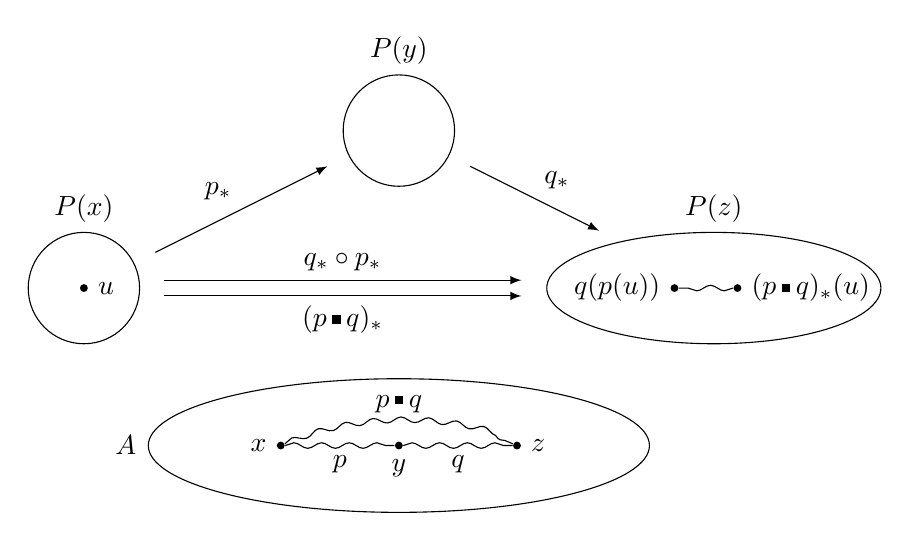
\begin{tikzpicture}[yscale=.5,xscale=1]
  \def\xshift{4}
  \def\yheight{4}

  % fibers
  \node[circle,draw,inner sep=0.5cm,label=above:{$P(x)$}] (px) at (-\xshift,\yheight) {};
  \node[circle,fill,inner sep=1pt,label=right:{$u$}] (u) at (px) {};

  \node[circle,draw,inner sep=0.5cm,label=above:{$P(y)$}] (py) at (0,2.0*\yheight) {};

  % P(z)
  \node[circle,draw,inner sep=0.5cm,label=above:{$P(z)$},xscale=3] (pz) at (\xshift,\yheight) {};
  \node[circle,fill,inner sep=1pt,label=left:{$q(p(u))$}] (qpu) at (\xshift-0.5,\yheight) {};
  \node[circle,fill,inner sep=1pt,label=right:{$(p\ct q)_\ast(u)$}] (pqu) at (\xshift+0.3,\yheight) {};
  \draw[decorate,decoration={snake,amplitude=1}] (pqu) -- (qpu);

  % paths
  \draw[->,shorten >=0.3cm,shorten <=0.3cm] (px) to[] node[auto] {$p_\ast$} (py) {};
  \draw[->,shorten >=0.3cm,shorten <=0.3cm] (py) to[] node[auto] {$q_\ast$} (pz) {};
  \draw[->,shorten >=0.3cm,shorten <=0.3cm, transform canvas={yshift=0.1cm}] (px) -- node[auto] {$q_\ast\circ p_\ast$} (pz) {};
  \draw[->,shorten >=0.3cm,shorten <=0.3cm, transform canvas={yshift=-0.1cm}] (px) -- node[below] {$(p\ct q)_\ast$} (pz) {};
 

  % Base space A
  \node[circle,draw,inner sep=0.5cm,label=left:{$A$},xscale=4.5,yscale=1.2] (A) at (0,0) {};
  \node[circle,fill,inner sep=1pt,label=left:{$x$}] (x) at (-1.5,0) {};
  \node[circle,fill,inner sep=1pt,label=below:{$y$}] (y) at (0,0) {};
  \node[circle,fill,inner sep=1pt,label=right:{$z$}] (z) at (1.5,0) {};
  \draw[decorate,decoration={snake,amplitude=1}] (x) -- node[auto,swap] {$p$} (y);
  \draw[decorate,decoration={snake,amplitude=1}] (y) -- node[auto,swap] {$q$} (z);
  \draw[decorate,decoration={snake,amplitude=1}] (x) to[bend left=40] node[auto] {$p\ct q$} (z);
\end{tikzpicture}
\end{document}